%Dokumentklasse
\documentclass[a4paper,12pt]{scrreprt}
\usepackage[top = 2.2 cm, left= 3.0 cm,right = 2cm, bottom = 2.8 cm]{geometry}
%\usepackage[onehalfspacing]{setspace}
% ============= Packages =============


% Dokumentinformationen
\usepackage[
	pdftitle={Titel der Abschlussarbeit},
	pdfsubject={},
	pdfauthor={Euer Name},
	pdfkeywords={},	
	%Links nicht einrahmen
	hidelinks
]{hyperref}


% Standard Packages
\usepackage{setspace}
\usepackage[utf8]{inputenc}
\usepackage[ngerman]{babel}
\usepackage[T1]{fontenc}
\usepackage{graphicx, subfig}
\graphicspath{{img/}}
%\usepackage{fancyhdr}
\usepackage{lmodern}
\usepackage{color}
\usepackage{tocbibind}




\usepackage{acronym}

% zusätzliche Schriftzeichen der American Mathematical Society
\usepackage{amsfonts}
\usepackage{amsmath}

%nicht einrücken nach Absatz
%\setlength{\parindent}{0pt}


% ============= Kopf- und Fußzeile =============
\usepackage{scrpage2}
\pagestyle{scrheadings}
\automark[section]{chapter}
\renewcommand*{\chapterpagestyle}{scrheadings}

\clearscrheadfoot

% Kopf aussen
\ohead{\headmark}   
% Kopf innen
\ihead{
\includegraphics[scale=0.15]{logo_esslingen.jpg}}  
\setheadsepline[text]{0.2pt}[]
% Fuß aussen
\ofoot[\pagemark]{\pagemark}   
% Fuß innen
\cfoot[]{Fabian Schirmer -- Digital Rights Management und Rechteübertragung} 




% ============= Package Einstellungen & Sonstiges ============= 
%Besondere Trennungen
\hyphenation{De-zi-mal-tren-nung}
\setlength{\parindent}{0pt}

% ============= Dokumentbeginn =============

\begin{document}
%Seiten ohne Kopf- und Fußzeile sowie Seitenzahl
\pagestyle{empty}

\begin{center}
\begin{tabular}{p{\textwidth}}


\begin{center}

\includegraphics[scale=0.5]{img/logo_esslingen.jpg}
\end{center}


\\

\begin{center}
\LARGE{\textsc{
Forschungsarbeit
}}
\end{center}

\\




\\

\begin{center}
\textbf{\Large{Digital Rights Management und Rechteübertragung}}
\end{center}

\begin{center}
Konzept für die Umsetzung und Kontrolle der rechtmäßigen Nutzung digitaler Medien auf Basis der Technologie Blockchain.
\end{center}

\\
\\
\begin{center}
\large{Fakultät Informatik \\
der Hochschule Esslingen \\}
\end{center}
\\

\begin{center}
vorgelegt von
\end{center}

\begin{center}
\large{\textbf{Fabian Schirmer}} \\
\small{Matrikelnummer: 759951}
\end{center}

\begin{center}
\large{Abgabetermin: DD.MM.JJJJ}
\end{center}

\\
\\
\\

\begin{center}
\begin{tabular}{lll}
\textbf{Betreuer:} & & Prof. Dr. Peter Väterlein\\
\textbf{Berater:} & &Rechtsanwalt Dr. Sascha Theißen\\
& &(Fachanwalt für Urheber- und It-Recht)
\end{tabular}
\end{center}

\end{tabular}
\end{center}


\pagestyle{scrheadings}
\pagenumbering{Roman}
\addchap{Eidesstattliche Erklärung}
\label{erklaerung}

Hiermit versichere ich, die vorliegende Abschlussarbeit selbstständig und nur unter Verwendung der von mir angegebenen Quellen und Hilfsmittel verfasst zu haben. Sowohl inhaltlich als auch wörtlich entnommene Inhalte wurden als solche kenntlich gemacht. Die Arbeit hat in dieser oder vergleichbarer Form noch keinem anderem Prüfungsgremium vorgelegen. \\
\\[1.5cm]
Datum:	\hrulefill\enspace Unterschrift: \hrulefill
\\[3.5cm]

\newpage
\addchap{Danksagung}
\label{danksagungen}
Mein besonderer Dank geht an Professor Dr. Peter Väterlein sowie Dr. Sascha Theißen für die technische Unterstützung, womit Sie mir bei der Konzeption und Durchführung dieser Arbeit wesentlich geholfen haben. Die Kooperation war nicht nur wissenschaftlich, sondern auch menschlich sehr fördernd für diese Arbeit. 



\addchap{Zusammenfassung}
\label{Zusammenfassung}


\minisec{Abstract}
\label{abstract}






% Beendet eine Seite und erzwingt auf den nachfolgenden Seiten die Ausgabe aller Gleitobjekte (z.B. Abbildungen), die bislang definiert, aber noch nicht ausgegeben wurden. Dieser Befehl fügt, falls nötig, eine leere Seite ein, sodaß die nächste Seite nach den Gleitobjekten eine ungerade Seitennummer hat. 
\cleardoubleoddpage

% pagestyle für gesamtes Dokument aktivieren

%Inhaltsverzeichnis
\tableofcontents
\newpage

\addchap{Abkürzungsverzeichnis}
\label{sec:abkuerzungsverzeichnis}


\begin{acronym}[KDE]
\acro{KDE}{K Desktop Environment}
\acro{Bash}{Bourne again shell}
\end{acronym}

\newpage
%Verzeichnis aller Bilder
\listoffigures


%Verzeichnis aller Tabellen
\listoftables

\newpage

\pagestyle{scrheadings}
\pagenumbering{arabic}

\chapter{Einleitung}
\label{sec:einleitung}
\begin{spacing}{1.5}
Der Wandel vom Industriezeitalter zum Digitalzeitalter schreitet immer schneller voran. Dies macht sich nicht nur im geschäftlichen sondern auch im privaten Umfeld bemerkbar. Digitale Medien gewinnen mehr und mehr die Oberhand. Dies ruft gleichzeitig kriminelle Handlungen auf den Plan. 
Diese Arbeit versucht einen Lösungsweg für diese Problematik zu arbeiten und eine sichere Methode vorzustellen, welche Langfristig eine Sicherheit bietet.
So lässt sich durch Studium dieser Arbeit  

\end{spacing}


\section{Motivation}
\label{sec:Motivation}
\begin{spacing}{1.5}
Derzeit befinden sich auf dem Markt sehr viele proprietäre Systeme, welche DRM (Digital Rights Management) zum Schutz digitaler Medien anbieten. Allerdings sind solche Anwendungen zum einen sehr einschränkend für den Benutzer. Das beutet entweder die Beschränkung auf eine bestimmte Hardware oder die Einschränkung des Nutzungsverhaltens.  
\end{spacing}


\section{Ziel der Arbeit}
Ziel dieser Arbeit ist es ein Konzept aufzuzeigen welches einen Mehrwert für die Verlage und für den jeweiligen Nutzer bietet. Dabei werden die Stichworte Sicherheit und gleichzeitige Anonymität auf Basis des juristischen Kontextes beachtet. 
\label{sec:Ziel der Arbeit}
\begin{spacing}{1.5}

\end{spacing}


\section{Überblick}
\label{sec:Überblick}
\begin{spacing}{1.5}

\end{spacing}

\chapter{Vorbetrachtungen und Grundlagen}
\label{sec:Vorbetrachtungen und Grundlagen}
\begin{spacing}{1.5}
In den nachfolgenden Punkten erfolgt eine Definition, Einordnung und interdisziplinäre Betrachtung der digitalen Rechteverwaltung. Im Kontext dazu werden das gesellschaftliche und juristische Umfeld näher beleuchtet. 

\section{Begriffsdefinition Digital Rights Management}
\label{sec:Begriffsdefinition Digital Rights Management}
Bevor mit der eigentlichen Betrachtung von Digital Rights Management(DRM) begonnen wird, ist eine einleitende Definition zum besseren Verständnis aufgeführt. Das Konzept DRM umfasst sogenannte Nutzungsregeln für ein digitales Objekt. Dabei umfasst der Begriff digitales Objekt alle möglichen digitalen Informationsmedien wie beispielsweise Bilder, eBooks usw. Die Nutzungsparameter umfassen dabei folgende Einschränkungen:

\begin{itemize}
\item \textit{Wer} ist berechtigt die digitalen Inhalte zu nutzen?
\item \textit{Wann} und \textit{Wo} werden die digitalen Inhalte genutzt?
\item \textit{Wie} wird das digitale Medium benutzt?
\end{itemize}

Dabei beinhaltet \textit{Wer} den Nutzungsberechtigten für das digitale Objekt, \textit{Wann} den Nutzungszeitraum(zeitlich begrenzte oder unbegrenzte Leihe) und \textit{Wo} definiert das autorisierte Abspielmedium. Das \textit{Wie} weißt beispielsweise Schreibrechte oder ausschließlich Leserechte dem Berechtigten zu. \cite [S.227]{DRM} \\
Neben dem Aufstellen der spezifischen Nutzungsregeln ist aber auch die Überwachung und Einhaltung dieser Parameter ein elementarer Bestandteil solcher Systeme. Dies wird zumeist von proprietärer Software übernommen, die die Einhaltung der Nutzungsbedingungen für das digitale Objekt gewährleistet.   

\section{Aufbau von DRM Systemen}
\label{Architektonischer Aufbau von DRM Systemen} 
Um ein besseres Verständnis über die Abläufe innerhalb eines DRM-basierten Systems zu bekommen, wird im Folgenden der grundsätzliche Aufbau solcher Systeme erläutert. 

\begin{figure}[ht]
\centering
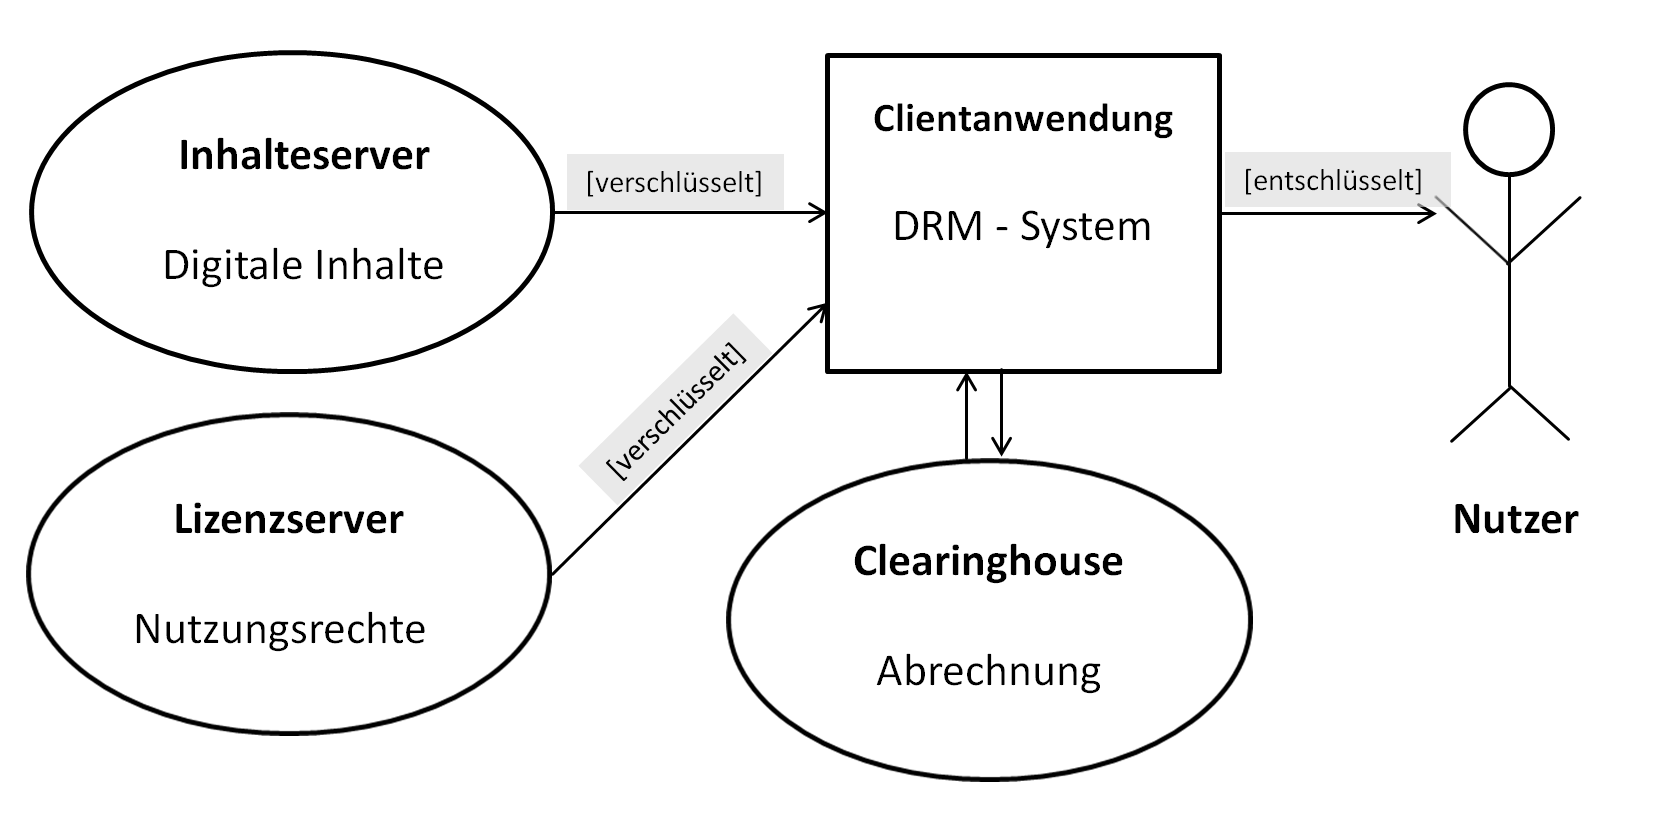
\includegraphics[scale=0.7]{img/DRM_Architektur}
\caption{DRM Ablaufschema}
\label{fig:DRM_Schema}
\end{figure}

Dieser Prozess, welcher in Abbildung \ref{fig:DRM_Schema} zu sehen ist, gliedert sich in drei Kernelemente. Um den architektonischen Aufbau derzeitiger Systeme zu verstehen, werden diese Kernelemente kurz vorgestellt. 
\begin{itemize}
\item \textbf{Inhalteserver} \\
Der Inhalteserver stellt das digitale Objekt in verschlüsselter Form zur Verfügung. 
\item \textbf{Lizenzserver} \\
Der Lizenzserver stellt die Nutzungsregeln für das digitale Objekt in verschlüsselter Form zur Verfügung. Diese können in feingranular unterteilt werden. Nähre Informationen sind unter 2.8 zu finden.  


\item \textbf{Clientanwendung} \\
Die Clientanwendung ist ein proprietäres System, welches das chiffrierte digitale Objekt und die jeweiligen Nutzungsrechte verarbeitet. Basierend auf den Nutzungsregeln wird das entschlüsselte digitale Objekt dem Anwender zur Verfügung gestellt. Jeglicher Fehlgebrauch, der nicht auf den Nutzungsregeln basiert, wird unterbunden. 
\end{itemize}

Um die Digital Rights Management Systeme auch aus kommerzieller Sicht zu komplementieren wird eine sogenanntes \textit{Clearinghouse} in das Gesamtkonstrukt eingebettet. Dieses übernimmt den Zahlungsvorgang. Dabei werden nachträgliche Erweiterung im Nutzungsrecht ebenfalls über diese Stelle abgewickelt \cite[S.151]{Architektur}. Nähere Informationen zum ökonomischen Standpunkt sind unter 2.8 aufgelistet. \\

!!Aüßere Form + Zitatquelle überprüfen

Neben der allgemeinen Definition haben sich zwei spezialisierte Konzepte der Digitalen Rechteverwaltung herausgebildet, die im nachfolgenden kurz vorgestellt werden.  


\section{Hard Weight DRM}
Der zuvor geschilderte Aufbau eines DRM-Systems wird auch als \textit{Hard DRM} bezeichnet. Dieses umfasst alle proprietären Systeme, die auf eine strikte Einhaltung der Nutzungsrechte beharren. Das digitale Objekt kann nur in der Art und Weise genutzt werden, wie es in den dazugehörigen Nutzungsregeln hinterlegt ist. Somit werden nur autorisierte Benutzer Zugang zum digitalen Medium gewährt. Gleichzeitig wird eine Autorisierung durchgeführt, die den Aktionsumfang für den Benutzer festlegt und somit entsprechend einschränkt. Möchte man den Umfang der Aktionen erweitern, kann dies durch Kauf zusätzlicher Nutzungsregeln initiiert werden \cite[S.335]{TypesOfDRM}. \\
Starke Einschränkungen rufen immer wieder illegale Machenschaften in den Fokus. Aufgrund dessen haben sich Industrie und Wissenschaft mit Alternativlösungen auseinandergesetzt.  
\label{sec: Hard Weight DRM}


\section{Light Weight DRM}
\label{sec:Light Weight DRM}
Der Gedanke hinter der sogenannten \textit{leichten digitalen Rechteverwaltung} ist ein Verzicht das Beharren auf Einhaltung der Nutzungsbestimmungen. Somit werden dem Endverbraucher mehr Freiheiten gewährt, was zu einer größeren Akzeptanz führt. \\
Jedes erworbene digitale Gut wird mit einer digitalen Signatur dem Benutzer zugeordnet. Die digitale Signatur ist wie eine Unterschrift in der analogen Welt anzusehen. Dieses Verfahren verursacht keinerlei Einschränkungen bei der Nutzung. Wird allerdings gegen die Nutzungsregeln verstoßen, so kann eindeutig nachgewiesen werden, wer gegen diese verstoßen hat. Mit diesem Wissen können im Nachhinein strafrechtliche Verfolgungen eingeleitet werden. \\
Um für die Konsumenten einen Anreiz zu schaffen, dass jeweilige digitale Produkt mittels Superdistribution\footnote{\label{foot:2}Verbreitung von chiffrierten digitalen Objekten unter den Benutzern über das Internet, Bluetooth oder sonstige standardisierte Übertragungswege \cite{Superdistribution}} weiterzuverbreiten, ist das \textit{PotatoSystem} entwickelt worden. Dieses begünstigt  


\cite[S. 90 ff.]{LightWeightDRM}



\section{Anforderungen an DRM}
\label{sec: Anforderungen an DRM}
\subsection{Authentifikaiton}
\label{Authentifikation}
\subsection{Autorisierung}
\label{Autorisierung}

\section{Juristische Betrachtung}
Digital Rights Management Systeme bewegen sich in einen schwierigen Terrain. Nicht zuletzt das es sich bei digitalen Objekten um immaterielle, nicht greifbare Gegenstände handelt. 
\label{sec:Juristische Betrachtung}
\subsection{Recht auf Löschung der Daten}
\label{Recht auf Löschung der Daten}
\subsection{Recht auf Privatkopie}
\label{Recht auf Privatkopie}
\subsection{Datenschutzgrundverordnung}
\label{Datenschutzgrundverordnung}
\subsection{Urheberrecht}
\label{Urheberrecht}

\section{Gesellschaftliche Betrachtung}
\label{sec:Gesellschaftliche Betrachtung}

\section{Ökonomische Betrachtung}
\begin{enumerate}
\item passive Nutzungsbestimmungen
	\begin{itemize}
	\item Zeitraumbegrenzung
	\item Anzahl der Nutzungen
	\item Länderbeschränkung
	\end{itemize}
\item aktive Nutzungbestimmungen
	\begin{itemize}
	\item Leserechte
	\item bestimmte Anzahl von Druckkopien
	\item Schreibrechte
	\end{itemize}
\item Nutzungsberechtigte
	\begin{itemize}
	\item eindeutige Benutzerzuweisung
	\item eindeutige Gerätezuweisung
	\end{itemize}
\end{enumerate} 

https://onlinelibrary.wiley.com/doi/pdf/10.1002/spe.2479
Eventuell eigene Grafik erstellen


\label{Ökonomische Betrachtung}

\section{Bestehende Probleme}
\label{sec:Bestehende Probleme}
Vorangegange Betrachtungen haben das generelle Bild der digitalen Rechteverwaltung zum einen klar definiert. Zum anderen wurde eine gesellschaftliche und juristische Einordnung vorgestellt, die das Gesamtbild abrundet. 

\end{spacing}


\chapter{Stand der Technik}
\label{cha:stand_der_technik}

\section{DRM Architekur}
\label{subsec:DRM Architektur}

\section{Verschlüsselung}
\label{Verschlüsselung}

\section{Digitale Wasserzeichen}
\label{Digitales Wasserzeichen}

\section{Trusted Computing}
\label{Trusted Computing}

\section{Rechtedefinitionssprachen}
\label{Rechtedefinitionssprachen}



\chapter{Konzept auf Basis der Technologie Blockchain}
\label{chap:entwicklung}

\section{Themenbezogene Veröffentlichungen}
\label{sec:themenbezogene_veroeffentlichungen}


\section{Funktionsweise}
\label{sec:grobkonzept}

\chapter{Ergebnisse}
\label{sec:ergebnisse}


\chapter{Diskussion}
\label{sec:diskussion}

\section{Zusammenfassende Bewertung}
\label{sec:überschrift}

\section{Ausblick}
\label{sec:ausblick}

%Literaturverzeichnis
\bibliographystyle{apalike} %alpha 
\bibliography{Literatur}

\end{document}
